\documentclass{article}

% if you need to pass options to natbib, use, e.g.:
% \PassOptionsToPackage{numbers, compress}{natbib}
% before loading nips_2016
%
% to avoid loading the natbib package, add option nonatbib:
% \usepackage[nonatbib]{nips_2016}

%\usepackage{nips_2016}

% to compile a camera-ready version, add the [final] option, e.g.:
 \usepackage[final]{nips_2016}

\usepackage[utf8]{inputenc} % allow utf-8 input
\usepackage[T1]{fontenc}    % use 8-bit T1 fonts
\usepackage{hyperref}       % hyperlinks
\usepackage{url}            % simple URL typesetting
\usepackage{booktabs}       % professional-quality tables
\usepackage{amsfonts}       % blackboard math symbols
\usepackage{nicefrac}       % compact symbols for 1/2, etc.
\usepackage{microtype}      % microtypography
\usepackage{amsmath}
\usepackage{fancyvrb}
\usepackage{algorithm}
\usepackage{algorithmic}
\usepackage{times}
% For figures
\usepackage{graphicx} % more modern
\usepackage{listings}
\graphicspath{{./img/}}
%\usepackage{epsfig} % less modern
\usepackage{subfigure} 
%\usepackage{subcaption}
% For citations
\usepackage{natbib}

\usepackage{amsmath, amsthm, amssymb, multirow, paralist}
\newtheorem{thm}{Theorem}
\newtheorem{prop}{Proposition}
\newtheorem{lemma}{Lemma}
\newtheorem{cor}{Corollary}
\newtheorem{definition}{Definition}
%\newtheorem{ass}[thm]{Assumption}
\newtheorem{assumption}{Assumption}
\newtheorem{obs}{Observation}

\usepackage{enumitem}
\usepackage{booktabs}     
\def \S {\mathbf{S}}
\def \A {\mathcal{A}}
\def \X {\mathcal{X}}
\def \Ab {\bar{\A}}
\def \R {\mathbb{R}}
\def \Kt {\widetilde{K}}
\def \k {\mathbf{k}}
\def \w {\mathbf{w}}
\def \v {\mathbf{v}}
\def \t {\mathbf{t}}
\def \x {\mathbf{x}}
\def \Se {\mathcal{S}}
\def \E {\mathrm{E}}
\def \Rh {\widehat{R}}
\def \x {\mathbf{x}}
\def \p {\mathbf{p}}
\def \a {\mathbf{a}}
\def \diag {\mbox{diag}}
\def \b {\mathbf{b}}
\def \e {\mathbf{e}}
\def \ba {\boldsymbol{\alpha}}
\def \c {\mathbf{c}}
\def \tr {\mbox{tr}}
\def \d {\mathbf{d}}
\def \z {\mathbf{z}}
\def \s {\mathbf{s}}
\def \bh {\widehat{b}}
\def \y {\mathbf{y}}
\def \u {\mathbf{u}}
%\def \L {\mathcal{L}}
\def \H {\mathcal{H}}
\def \g {\mathbf{g}}
\def \F {\mathcal{F}}
\def \I {\mathbb{I}}
\def \P {\mathcal{P}}
\def \Q {\mathcal{Q}}
\def \xh {\widehat{\x}}
\def \wh {\widehat{\w}}
\def \ah {\widehat{\alpha}}
\def \Rc {\mathcal R}

\def \Bh {\widehat B}
\def \Ah {\widehat A}
\def \Uh {\widehat U}
\def \Ut {\widetilde U}
\def \B {\mathbf B}
\def \C {\mathbf C}
\def \U {\mathbf U}
\def \Kh {\widehat K}
\def \fh {\widehat f}
\def \yh {\widehat y}
\def \Xh {\widehat{X}}
\def \Fh {\widehat{F}}


\def \y {\mathbf{y}}
\def \E {\mathrm{E}}
\def \x {\mathbf{x}}
\def \g {\mathbf{g}}
\def \D {\mathcal{D}}
\def \z {\mathbf{z}}
\def \u {\mathbf{u}}
\def \H {\mathcal{H}}
\def \Pc {\mathcal{P}}
\def \w {\mathbf{w}}
\def \r {\mathbf{r}}
\def \R {\mathbb{R}}
\def \S {\mathcal{S}}
\def \regret {\mbox{regret}}
\def \Uh {\widehat{U}}
\def \Q {\mathcal{Q}}
\def \W {\mathcal{W}}
\def \N {\mathcal{N}}
\def \A {\mathcal{A}}
\def \q {\mathbf{q}}
\def \v {\mathbf{v}}
\def \M {\mathcal{M}}
\def \c {\mathbf{c}}
\def \ph {\widehat{p}}
\def \d {\mathbf{d}}
\def \p {\mathbf{p}}
\def \q {\mathbf{q}}
\def \db {\bar{\d}}
\def \dbb {\bar{d}}
\def \I {\mathcal{I}}
\def \xt {\widetilde{\x}}
\def \f {\mathbf{f}}
\def \a {\mathbf{a}}
\def \b {\mathbf{b}}
\def \ft {\widetilde{\f}}
\def \bt {\widetilde{\b}}
\def \h {\mathbf{h}}
\def \B {\mathbf{B}}
\def \bts {\widetilde{b}}
\def \fts {\widetilde{f}}
\def \Gh {\widehat{G}}
\def \G {\mathcal {G}}
\def \bh {\widehat{b}}
\def \fh {\widehat{f}}
\def \wh {\widehat{\w}}
\def \vb {\bar{v}}
\def \zt {\widetilde{\z}}
\def \zts {\widetilde{z}}
\def \s {\mathbf{s}}
\def \gh {\widehat{\g}}
\def \vh {\widehat{\v}}
\def \Sh {\widehat{S}}
\def \rhoh {\widehat{\rho}}
\def \hh {\widehat{\h}}
\def \C {\mathcal{C}}
\def \V {\mathcal{L}}
\def \t {\mathbf{t}}
\def \xh {\widehat{\x}}
\def \Ut {\widetilde{U}}
\def \wt {\widetilde{\w}}
\def \Th {\widehat{T}}
\def \Ot {\tilde{\mathcal{O}}}
\def \X {\mathcal{X}}
\def \nb {\widehat{\nabla}}
\def \K {\mathcal{K}}
\def \P {\mathbb{P}}
\def \T {\mathcal{T}}
\def \F {\mathcal{F}}
\def \ft{\widetilde{f}}
\def \xt {\widetilde{x}}
\def \Rt {\mathcal{R}}
\def \Rb {\bar{\Rt}}
\def \wb {\bar{\w}}
\title{Efficient Distributed Stochastic Dual Coordinate Ascent}

% The \author macro works with any number of authors. There are two
% commands used to separate the names and addresses of multiple
% authors: \And and \AND.
%
% Using \And between authors leaves it to LaTeX to determine where to
% break the lines. Using \AND forces a line break at that point. So,
% if LaTeX puts 3 of 4 authors names on the first line, and the last
% on the second line, try using \AND instead of \And before the third
% author name.

\author{
  Mingrui Liu, Jeff Hajewski \\
  Department of Computer Science\\
  University of Iowa\\
  Iowa City, IA  52242 \\
  \texttt{mingrui-liu@uiowa.edu, jeffery-hajewski@uiowa.edu} \\
  %% examples of more authors
%   \And
%   123\\Department of Computer Science\\
%   	University of Iowa\\
%   	Iowa City, IA  52242 \\
%   	\texttt{mingrui-liu@uiowa.edu, jeffery-hajewski@uiowa.edu} \\
  %%Affiliation{Department of Computer Science} \\
  %% Address \\
  %% \texttt{email} \\
  %% \AND
  %% Coauthor \\
  %% Affiliation \\
  %% Address \\
  %% \texttt{email} \\
  %% \And
  %% Coauthor \\
  %% Affiliation \\
  %% Address \\
  %% \texttt{email} \\
  %% \And
  %% Coauthor \\
  %% Affiliation \\
  %% Address \\
  %% \texttt{email} \\
}

\begin{document}
% \nipsfinalcopy is no longer used

\maketitle

\begin{abstract}
%  The abstract paragraph should be indented \nicefrac{1}{2}~inch
%  (3~picas) on both the left- and right-hand margins. Use 10~point
%  type, with a vertical spacing (leading) of 11~points.  The word
%  \textbf{Abstract} must be centered, bold, and in point size 12. Two
%  line spaces precede the abstract. The abstract must be limited to
%  one paragraph. This latex file is modified from the NIPS  2016 template. 
We propose the design and analysis of an efficient, distributed, 
SDCA algorithm that uses GPUs to improve computational efficiency for parameter updates. This work builds off the previous work of T.
Yang \cite{yang2013trading}, 
%M. Li \cite{li2014scaling}, and A. Agarwal
%\cite{agarwal2011distributed}
 creating a more scalable and efficient SDCA
algorithm. Specifically, we propose to use CUDA to improve the runtime
efficiency of the gradient and parameter update calculations %along with the use
%of MPI for network communication. 
The implementation is completely written in pure C++.
%The asynchronous nature of the communication
%will be handled using standard MPI facilities combined with threading in C++.
\end{abstract}

\section{Introduction}
%What is the research problem that you are trying to tackle? Describe the background and motivation. 
In recent years, the amount and size of available data has grown at an
incredible rate. As the size of the data grows, the challenge of applying
standard machine learning algorithms to the data has become increasingly
complex. Two common countermeasures used to deal with this are employing
stochastic optimization algorithms, and utilizing computational resources in a
parallel or distributed manner~\cite{boyd2011distributed}. 

In this paper, we consider a class of convex optimization problems with special
structure, whose objective can be expressed as the sum of a finite sum of loss
functions and a regularization function: \begin{equation}
\label{RLM}
	\min_{w\in\R^d}P(w), \text{where }P(w)=\frac{1}{n}\sum_{i=1}^{n}\phi(w^\top x_i,y_i)+\lambda g(w),
\end{equation}
where $w\in\R^d$ denotes the weight vector, $(x_i,y_i),x_i\in\R^d,y_i\in\R$,
$i=1,\ldots,n$ are training data, $\lambda>0$ is a regularization parameter,
$\phi(z,y)$ is a convex function of $z$, and $g(w)$ is a convex function of $w$.
We refer to the problem in (\ref{RLM}) as Regularized Finite Sum Minimization
(RFSM) problem. When $g(w)=0$, the problem reduces to the Finite Sum
Minimization (FSM) problem.

Both RFSM and FSM problems have been extensively studied in machine learning and
optimization literature. When $n$ is large, numerous sequential stochastic
optimization algorithms have been
proposed~\cite{bottou2010large,nemirovski2009robust,roux2012stochastic,shalev2013stochastic,shalev2013accelerated,johnson2013accelerating,ouyang2013stochastic,
suzuki2013dual,shalev2014accelerated,xiao2014proximal,defazio2014saga,zhang2015stochastic,lin2014accelerated,defazio2016simple,allen2016katyusha,lan2015optimal},
and there also exist several parallel or distributed stochastic
algorithms~\cite{boyd2011distributed,recht2011hogwild,zinkevich2010parallelized,yang2013trading,zhang2014asynchronous,zinkevich2010parallelized,agarwal2011distributed}.
Specifically, S. Shalv-Shwartz and T. Zhang~\cite{shalev2013stochastic} proposed
the Stochastic Dual Coordinate Ascent (SDCA) which provided new analysis with strong theoretical
guarantees regarding the duality gap. T. Yang~\cite{yang2013trading,yang2013analysis} developed two 
Distributed Stochastic Dual Coordinate Ascent (DisDCA) algorithms and analyzed
the tradeoff between network communication between nodes and the difficulty of
the performed computation (task). However, the problem of developing a more
efficient distributed SDCA algorithm is still open. In this paper, we first
provide a GPU implementation of the vanilla distributed
SDCA~\cite{yang2013trading}, and then give an asynchronous distributed approach
to SDCA to make full use of computational resources that scale well. 

\section{Related Work}
%\label{gen_inst}
First we review the related work of sequential stochastic convex optimization
for solving FSM and RFSM problems. The first numerical scheme of stochastic
optimization stems from stochastic gradient descent
(SGD)~\cite{bottou2010large,nemirovski2009robust}, which was designed to avoid
the calculation of full gradient and gets faster convergence than full gradient
descent (FGD). To improve the converge rate of SGD, many new algorithms were
proposed by exploiting the finite sum structure, including the Stochastic
average gradient (SAG)~\cite{roux2012stochastic}, stochastic dual coordinate
ascent (SDCA)~\cite{shalev2013stochastic}, stochastic variance reduced gradient
(SVRG)~\cite{johnson2013accelerating}, accelerated proximal coordinate gradient method
(APCG)~\cite{lin2014accelerated},  SAGA~\cite{Defazio2014},
Prox-SDCA~\cite{shalev2014accelerated}, Prox-SVRG~\cite{xiao2014proximal}, and
stochastic primal-dual coordinate method (SPDC)~\cite{zhang2015stochastic}.
Recently, the optimal first-order stochastic optimization method were
developed~\cite{allen2016katyusha,lan2015optimal}. Although there exist rich
literature studying sequential stochastic optimization with strong theoretical
guarantee, less efforts have been devoted to considering them in a parallel or
distributed manner. It constitutes a huge gap between theory and practice, since
nowadays the size of data increases at a rapid speed, which makes one-core
processor or one computer very difficult to handle it properly. 

Then we review several related work of distributed optimization algorithms. In
the existing literature, many distributed algorithms have been developed on top of
stochastic gradient descent (SGD), alternating direction method of multipliers
(ADMM), and stochastic dual coordinate ascent (SDCA). The two main approaches
used in developing parallel algorithsm for SGD are based on shared memory and
distributed memory architectures. Some work~\cite{lian2015asynchronous}
looks at both settings, in addition to removing the syncrhonization requirement
in the distributed memory setting.
A number of approaches~\cite{zinkevich2010parallelized,recht2011hogwild,agarwal2011distributed}
consider the asynchronous or lock-free setting, making use of parameter servers
\cite{li2014scaling}, sparsity \cite{recht2011hogwild}, as well as unique
data-flow architectures for parameter updates \cite{agarwal2011distributed}.
ADMM stems from \cite{gabay1976dual}, which was developed to solve the equality
constrained optimization problem. Recently, two independent works of stochastic
ADMM were proposed~\cite{ouyang2013stochastic,suzuki2013dual}. A standard
reference for distributed ADMM is~\cite{boyd2011distributed}. The advances of
SDCA algorithms~\cite{shalev2013stochastic} and its
variant~\cite{shalev2013accelerated,shalev2014accelerated,lin2014accelerated}
enjoy faster convergence than SGD and ADMM, and the distributed SDCA
(DisDCA)~\cite{yang2013trading,yang2013analysis} was developed along with novel
analysis of tradeoff between computation and communication. \cite{yang2013trading} serves as the starting point for our work.

%We will build off of work from T. Yang's work on distributed SDCA~\cite{yang2013trading}, first add GPU capabilities and then incorporating M.
%Li's work on parameter servers~\cite{li2014scaling} to handle communication
%updates in the distributed setting.  In~\cite{yang2013trading}, SDCA is
%implemented in a distributed, synchronized fashion. While the achieved results
%were quite promising, they did not take advantage of hardware acceleration or
%asynchronous communication.  \cite{li2014scaling} builds an asynchronous
%communication framework using the concept of parameter servers, which are
%central data stores for model parameters, and distributed workers working in an
%asynchronous fashion (i.e., communication and parameter updates are non-blocking
%operations).  Additionally,
%\cite{agarwal2011distributed} explores the
%theoretical ramifications of delayed parameter updates in general distributed
%stochastic optimization setting. By combining the work
%of T. Yang, M. Li, and A. Agarwal, we hope to develop a robust,
%distributed SDCA solution.

In~\cite{yang2013trading}, SDCA is
implemented in a distributed, synchronized fashion. While the achieved results
were quite promising, they did not take advantage of hardware acceleration or
asynchronous communication.  We will build off of work from T. Yang's work on distributed SDCA~\cite{yang2013trading}, and add GPU capabilities. 
\section{GPU Acceleration for Sequential SDCA}
\begin{algorithm}[H]
	\caption{Sequential SDCA}
	\label{sequentialSDCA}
	\begin{algorithmic}[1]
	\REQUIRE~~ $\alpha^{(0)}$
		\ENSURE~~$\bar{w}$
		\STATE Let $w^{(0)}=w(\alpha^{(0)})$, where $w(\alpha)=\frac{1}{n}\sum_{i=1}^{n}\alpha_ix_i$
		\FOR{ $t=1,2,\ldots,T$}
		\STATE Randomly pick $i$
		\STATE Find $\Delta\alpha_i$ to maximize $-\phi_i^*(-(\alpha^{(t-1)}+\Delta\alpha_i))-\frac{\lambda n}{2}\|w^{(t-1)}+(\lambda n)^{-1}\Delta \alpha_i x_i\|^2$
		\STATE $\alpha^{(t)}\leftarrow\alpha^{(t-1)}+\Delta\alpha_ie_i$
		
		\STATE $w^{(t)}\leftarrow w^{(t-1)}+(\lambda n)^{-1}\Delta\alpha_i x_i$
		\ENDFOR
		
		\STATE Output (Random option):\\
		Let $\bar{\alpha}=\alpha^{(t)}$ and $\bar{w}=w^{(t)}$ for some random $t\in T_0+1,\ldots,T$\\
		\RETURN $\bar{w}$
		
	\end{algorithmic}
\end{algorithm}
The traditional SDCA algorithm \cite{shalev2013stochastic} is described in Algorithm \ref{sequentialSDCA}, where $g(w)=\frac{1}{2}\|w\|_2^2$.
In that procedure, the most expensive work is in line 4--6. We employ the GPU acceleration technique to make those lines run in a faster manner.
\subsection{Naive GPU Implementation}
The naive implementation (hereafter referred to as the sequential GPU algorithm)
is simply the CPU-based algorithm but we replace all linear algebra/vector
operations with CUDA kernels and carrying them out on the GPU. In other words,
there is no change to the SDCA algorithm, we simply perform some of our
calculations on the GPU, rather than performing everything on the CPU.

\subsection{Refined GPU Implementation}
The refined GPU implementation improves upon the naive implementation by
optimizing memory allocations. This is done by using static pointers to hold the
address of the allocated memory on the GPU. Once this memmory is allocated,
there is no need to re-allocate, since we can access it via the pointers. The
memory is re-allocated only in the event that the amount of memory needed
changes.

\section{GPU Acceleration for Distributed SDCA}
The distributed SDCA \cite{yang2013trading} is described in Algorithm
\ref{distributedSDCA}. We restrict our implementation over the case when
$g(w)=\frac{1}{2}\|w\|_2^2$. The procedure \textbf{SDCA-mR} is the procedure on
$k$-th machine (process).

\begin{algorithm}[H]
	\caption{Distributed SDCA}
	\label{distributedSDCA}
	\begin{algorithmic}[1]
		\STATE	Start $K$ processes by calling the following procedure \textbf{SDCA-mR} with input $m$ and $T$.\\ 
		\begin{center}Procedure \textbf{SDCA-mR}
			\end{center}
		\REQUIRE~~Number of Iterations $T$, number of samples $m$ at each iteration
		\ENSURE~~$w^{T}$
	\STATE Let $\alpha_k^{(0)}=0$, $v^{(0)}=0$, $w^{0}=0$
	\STATE \textbf{Read Data:} $(x_{k,i},y_{k,i})$, $i=1,\ldots,n_k$
	\FOR{$t=1,\ldots,T$}
	\FOR{$j=1,\ldots,m$}
	\STATE Randomly pick $i\in\{1,\ldots,n_k\}$ and let $i_j=i$
	\STATE Find $\Delta\alpha_{k,i}$ by
	\begin{equation*}
		\Delta\alpha_{k,i}=\max_{\Delta\alpha}-\phi_{k,i}^*(-(\alpha_{k,i}^{t-1}+\Delta\alpha))-\Delta\alpha x_{k,i}^\top w^{t-1}-\frac{mK}{2\lambda n}(\Delta\alpha)^2\|x_{k,i}\|_2^2
	\end{equation*}
	\STATE Set $\alpha_{k,i}=\alpha_{k,i}^{t-1}+\Delta\alpha_{k,i}$
	\ENDFOR
	\STATE \textbf{Reduce:} $v^{t}:\frac{1}{\lambda n}\sum_{j=1}^{m}\Delta\alpha_{k,i_j}x_{k,i_j}\rightarrow v^{t-1}$\\ (Remark: the reduce step is implemented in two steps
	\begin{itemize}
		\item The master node adds the increment from each machine (process) together
		 \item Each machine (process) receives $v^t$ from the broadcasting process from master node 
		\end{itemize})
	\STATE \textbf{Update:} $w^t=v^t$
%	\STATE Wait for Other Machine updating $w^{t}$ and receive the updated $w^{(t)}$ from the master node, where the mas
	\ENDFOR
	\RETURN $w^T$
	\end{algorithmic}
\end{algorithm}
We took the idea of parallelizing SDCA over a number of machines,
and replaced the machines with threads on a GPU. Instead of network
communication we have communication via the PCIE bus, which, while slower than
RAM access, is considerably faster than ethernet. Additionally, rather than send
a batch of data to each thread (to mimic sending data to a worker node), we send
a single data point to $k$ threads, rather than $m$ data points to $k$ threads.
This simplifies communication and computation, and results ing a matrix-vector
calculation that is performed on the GPU. While we could further optimize this
algorithm by performing additional calculations on the GPU, the low-level
implementations and handling of shared and non-shared GPU memory as well as
thread synchronization proved to be too much to tackle for this project given
our time constraint. However, moving forward these are great areas to explore.

\section{Implementation}
%As seen in the preceding table and figure, 
In our experiments, we use $\phi(z,y)=\max(0,1-yz)$ and $\lambda=10$.
The CPU implementation outperformed
the GPU implementations across the board. While this was not expected, the
results are very interesting from an implementation point of view. There are a
few key areas that hurt the GPU implementation -- unfortunately we did not have
enough time to fix/implement these properly.
\begin{itemize}
	\item Memory allocation
	\item Device-host communication
	\item Optimized kernel implementations
\end{itemize}

\subsection{Memory Allocation}
This was the first issue we ran into during our work on the sequential GPU
algorithm (which we implmented prior to the distributed version). Our initial
implementation made no optimizations in terms of memory allocation. Each time
we performed any work on the GPU, we would allocate memory, transfer the data,
perform the operation, transfer the data bac, and the release the allocated
device memory. This resulted in over a million allocations on a small dataset
and made up about 13s of compute time for the same run. After profiling our
code using \texttt{nvprof} we realized the excessive allocations were really
degrading performance and largely unnecessary.\\

To fix this issue, we created static
pointers to allocated memory on the device. These pointers were allocated once,
reducing our device memory allocations from the millions down to just three
allocations (two allocations for vectors, and a third allocation for the
result). This was an immense savings, and reduce the compute time for the dot
product kernel from 13s down to less than a second for the test data set
(roughly 100 points in $\R^3$).\\

For the distributed version, we added two additional static pointers for a
matrix (which held the entire mini-batch) and a second result vector for the
result of a matrix-vector multiplication. 

\subsection{Device-Host Communication}
This is the second issue we ran into, but did not have enough time to correct.
Throughout our algorithm, we transfer data to and from the GPU each time we
encounter an operation that can be efficiently computed on the GPU. This means
there are situations where we transfer data to or from the GPU when we don't
necessarily need to -- either the data already resides on the GPU or we don't
actually need the result vector. Using \texttt{nvprof} we saw that
communication was now dominating our GPU compute time, consisting of nearly
50\% of total GPU compute time.\\

However, fixing this issue is quite a bit more complicated than fixing the
allocation issue mentioned in the previous section. There are two improvements
that can improve the communication between host and device: memory pinning and
warpping our data in a class that handles memory synchronization in the
background.

\paragraph{Memory Pinning} Memory pinning is declaring that the memory
allocations on the host (that are the source for the transfer to device) will
not be paged. This means the data stays in pinned memory so no transfer from
paged out memory to pinned memory is necessary (or even checking if it's
necessary). However, since we are using fairly modern hardware, the impact from
using pinned memory is not as significant as being more efficient with when we
transfer between host and device.

\paragraph{Data Wrapper} Creating a data wrapper around the data types we used
from Eigen would allow us to more intelligently handle transfers between host
and device. Specifically, we would be able to determine where the data is
currently located (device or host) and decide whether a transfer is needed or
not. For example, if the weight vector is currently sitting on the GPU, no
updates are made to the weights on the host, more data is transferred to the
GPU, we could avoid both a transfer of the weight from device to host and then
again from host to device by simply leaving the weight vector on the GPU.

\subsection{Optimized CUDA kernel implementations}
The last issue is the implementation of our CUDA kernels. The dot-product
kernel was fairly straightforward, but the matrix-vector kernel leaves room for
improvement. Overall, there are a large number of kernel optimizations that can
be made to improve overall kernel throughput, but these optimizations can be
very low-level. Using a library such as cuBLAS would have been a better
approach in hind-sight. However, at the onset of the project we determined
writing a wrapper class for our data that would allow us to interface with the
cuBLAS kernels more easily would require more time than we had available for
the project.\\

Aside from taking advantage of cuBLAS, we can also perform more operations in
the update phase of the distributed GPU algorithm on the GPU. Currently we
simply perform a matrix-vector multiplication and then handle everything else on
the host. By performing more of the update work on the GPU, we could squeeze
even more performance out of this approach.

\section{Experimental Results}
Our results were not as promising as we anticipated. Table \ref{tab:res-scale}
shows the results using a created data set in $\R^{100}$ that contained 10,000
data points. We ran three algorithms: sequential CPU, sequential GPU, and
distributed GPU. Sequential CPU is just the standard implementation of SDCA.
Sequential GPU extends this implementation by performing dot product operations
on the GPU. The distributed GPU version is the implementation of distributed
SDCA on the GPU (rather than a cluster). All algorithms were run for 5 epochs
without any type of early termination. We are measuring, roughly speaking, how
these algorithms compare in terms of the time it takes to complete a predefined
workload. As we will see in a later discussion, our algorithms also converge to
similar training losses.

\begin{table}
  \centering
  \caption{Results of sequential CPU, sequential GPU, and distributed GPU
    for a sample data set of 10,000 points each having 100 features. Times are
    given in MM:SS.}
  \label{tab:res-scale}
  \begin{tabular}{l|cccc}
      \textbf{Algorithm} & \textbf{mini-batch = 1} & \textbf{mini-batch = 32} &
      \textbf{mini-batch = 64} & \textbf{mini-batch = 128}\\\hline
      Sequential CPU & 7:36 & 0:23 & 0:16 & 0:13\\
      Sequential GPU & 7:50 & 0:25 & 0:19 & 0:15\\
      Distributed GPU & 33:33 & 1:10 & 0:40 & NA\\\hline
  \end{tabular}
\end{table}

Sequential CPU outperformed both GPU implementations due to implementation
issues. However, as expected, the distributed GPU version improved in terms of
compute time as the size of the mini-batch increased. As the mini-batch size
increases, the number of coordinate directions optimized in the distributed
SDCA algorithm increases, and these optimizations are done in parallel on the
GPU. Performing more of these updates simultaneously on the GPU reduces the
number of communications with the GPU and thus improving  the overall runtime.
Conversely, as the mini-batch size decreases we would expect GPU compute times
to degrade, since a small mini-batch requires more data transfers back and
forth between host RAM (on the computer) and device RAM (VRAM on the
GPU). Lastly, the NA result for the distributed GPU implementation on a batch
size of 128 is the result of a memory corruption error. At the time of writing
this report we were still chasing down the cause of the memory corruption. We
believe this is a bad memory access while indexing through the matrix of data on
the GPU, but are still working on this issue. As we will discuss later, this is
another reason we would have been better off using a third-party library for
these kernels (such as cuBLAS, implemented by NVIDIA).\\

Figure \ref{fig:australian} shows a graph comparing sequential CPU versus
sequential GPU for the Australian dataset (from the LibSVM data archives). This
data set only contains 54 features and roughly 690 data points, making it a good
data set for quick tests and analyses.

\begin{figure}
  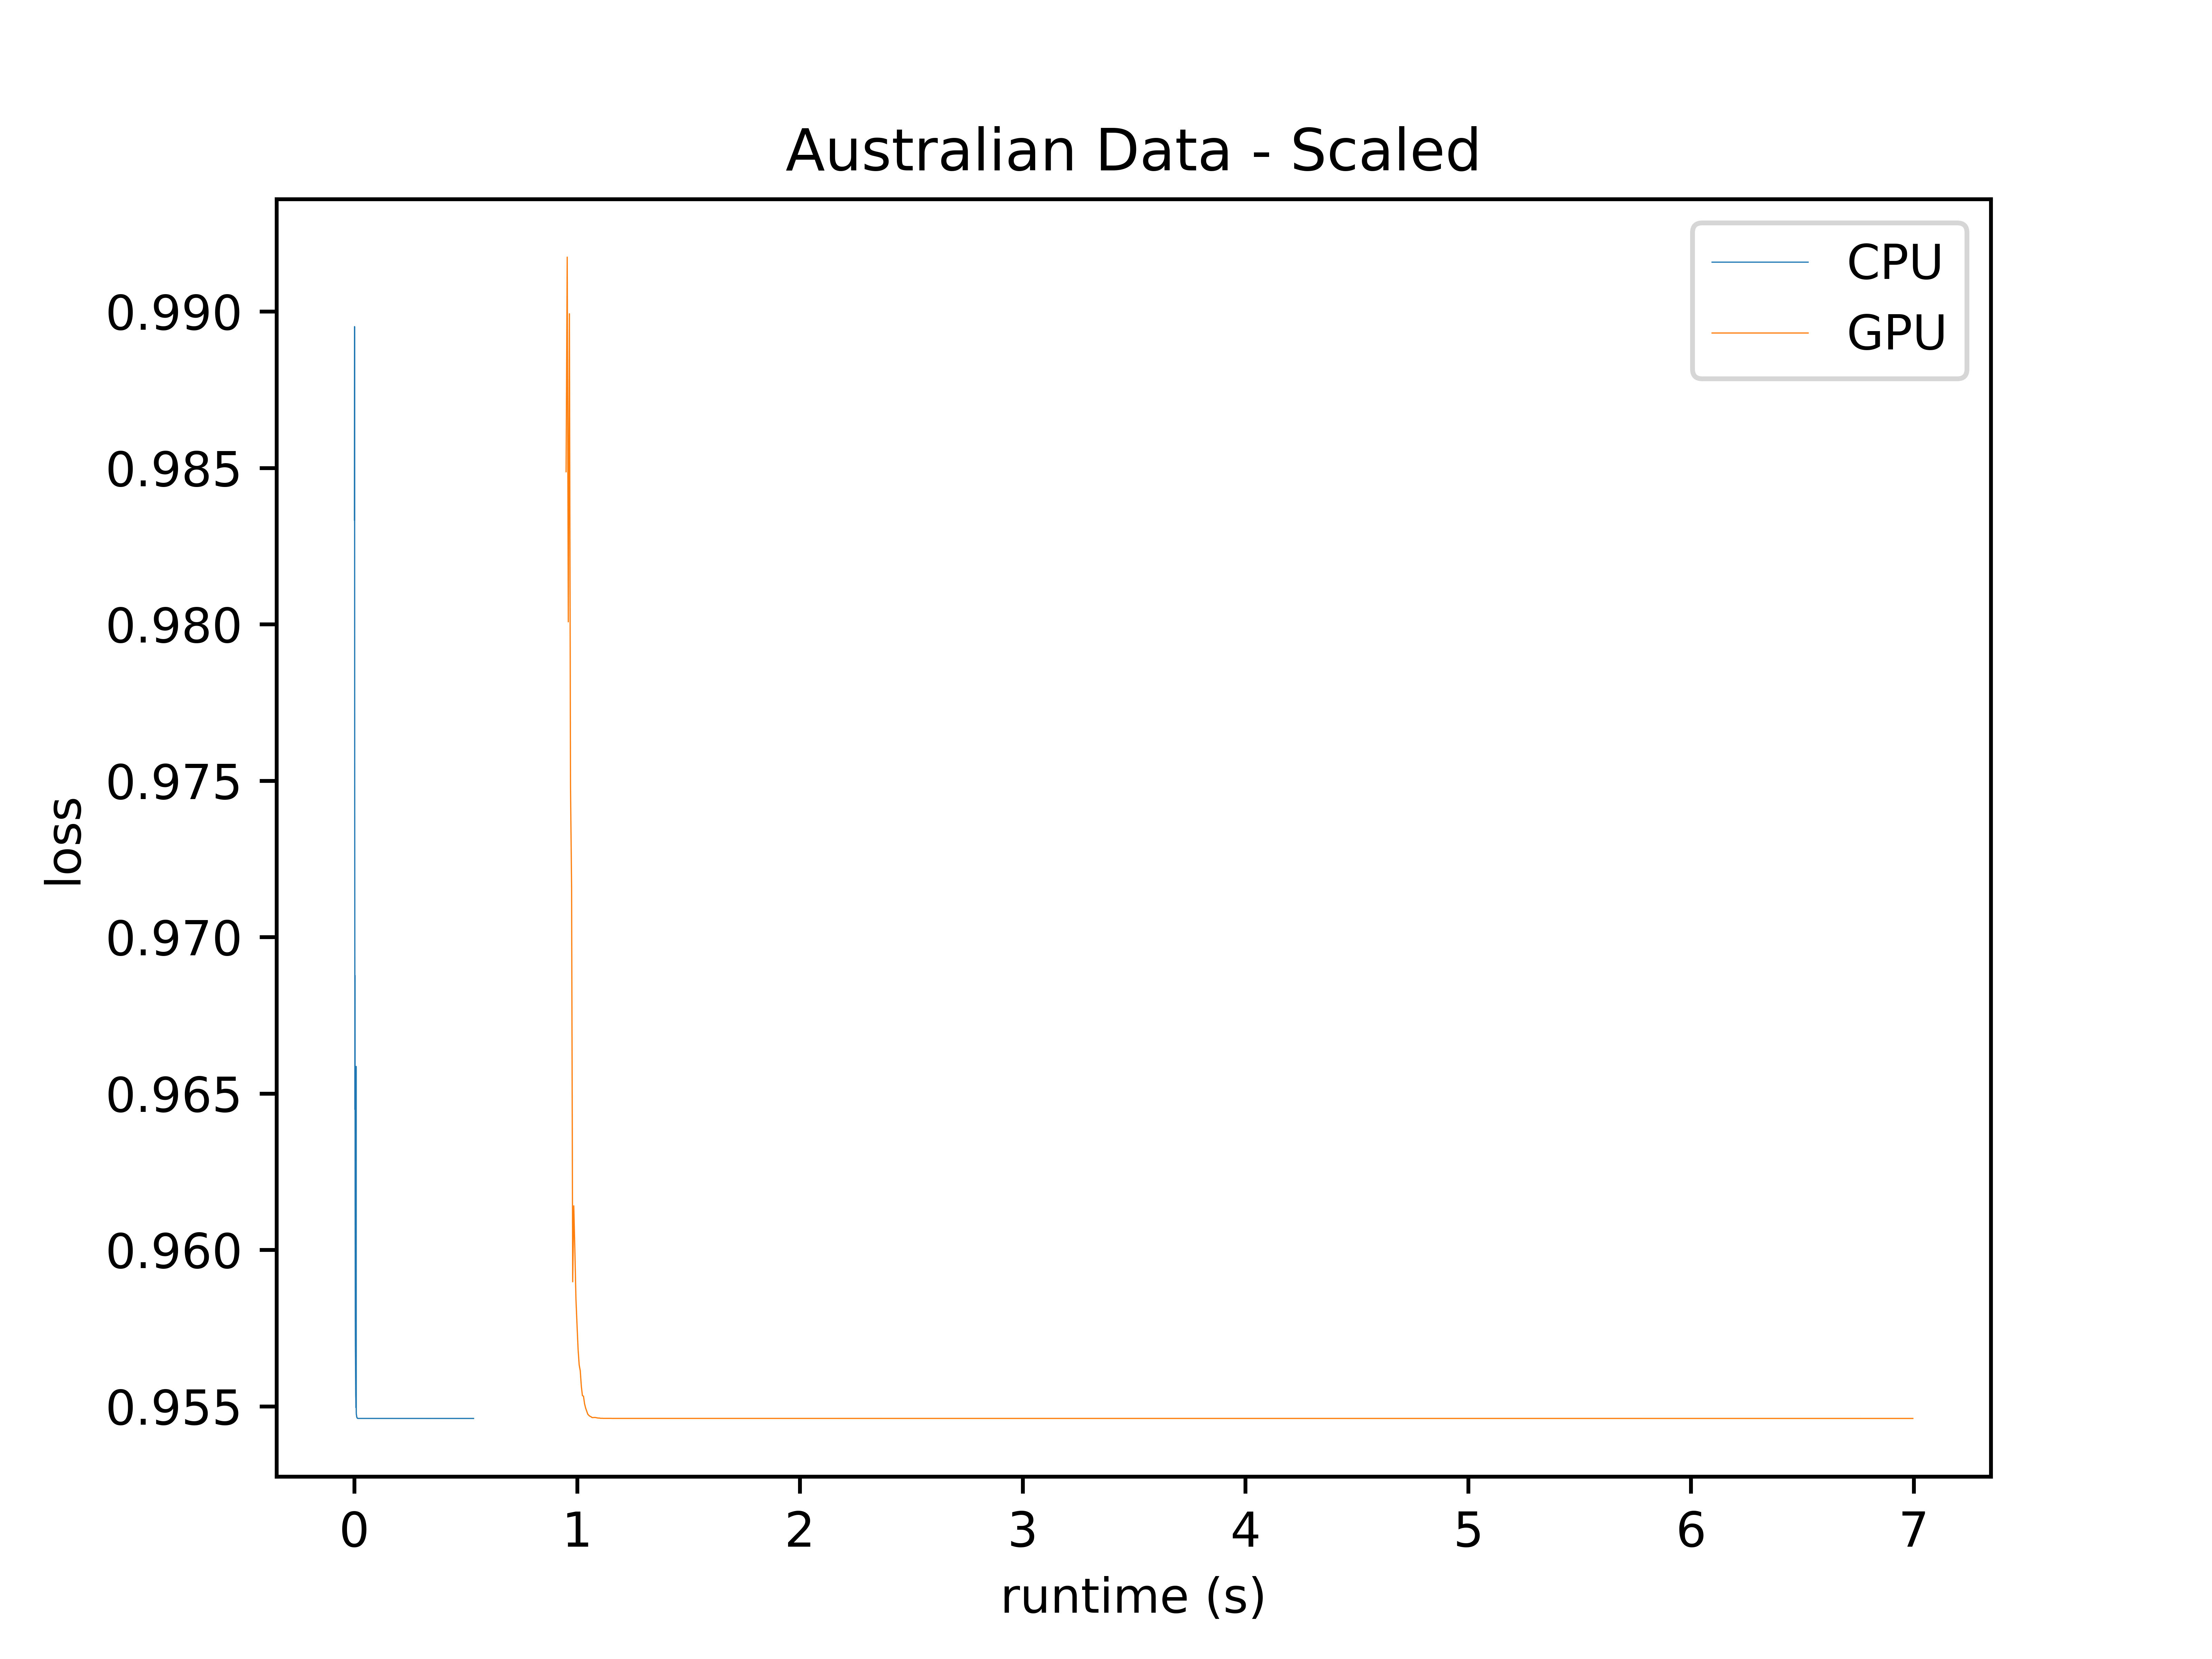
\includegraphics[scale=0.5]{cpu_vs_gpu}
  \centering
  \caption{Comparison of training loss for sequential CPU and sequential GPU for
    the scaled Australian data set.}
  \label{fig:australian}
\end{figure}

To get a better sense of the CPU versus GPU comparison, we generated data that
would allow us to control the number of features so we could better understand
how more features impacted performace on the GPU and CPU implementations. Figure
\ref{fig:10k} shows a comparison of sequential CPU versus sequential GPU for
data with 10,000 features while Figure \ref{fig:50k} shows the same comparison
but for data with 50,000 features.

\begin{figure}
  \centering
  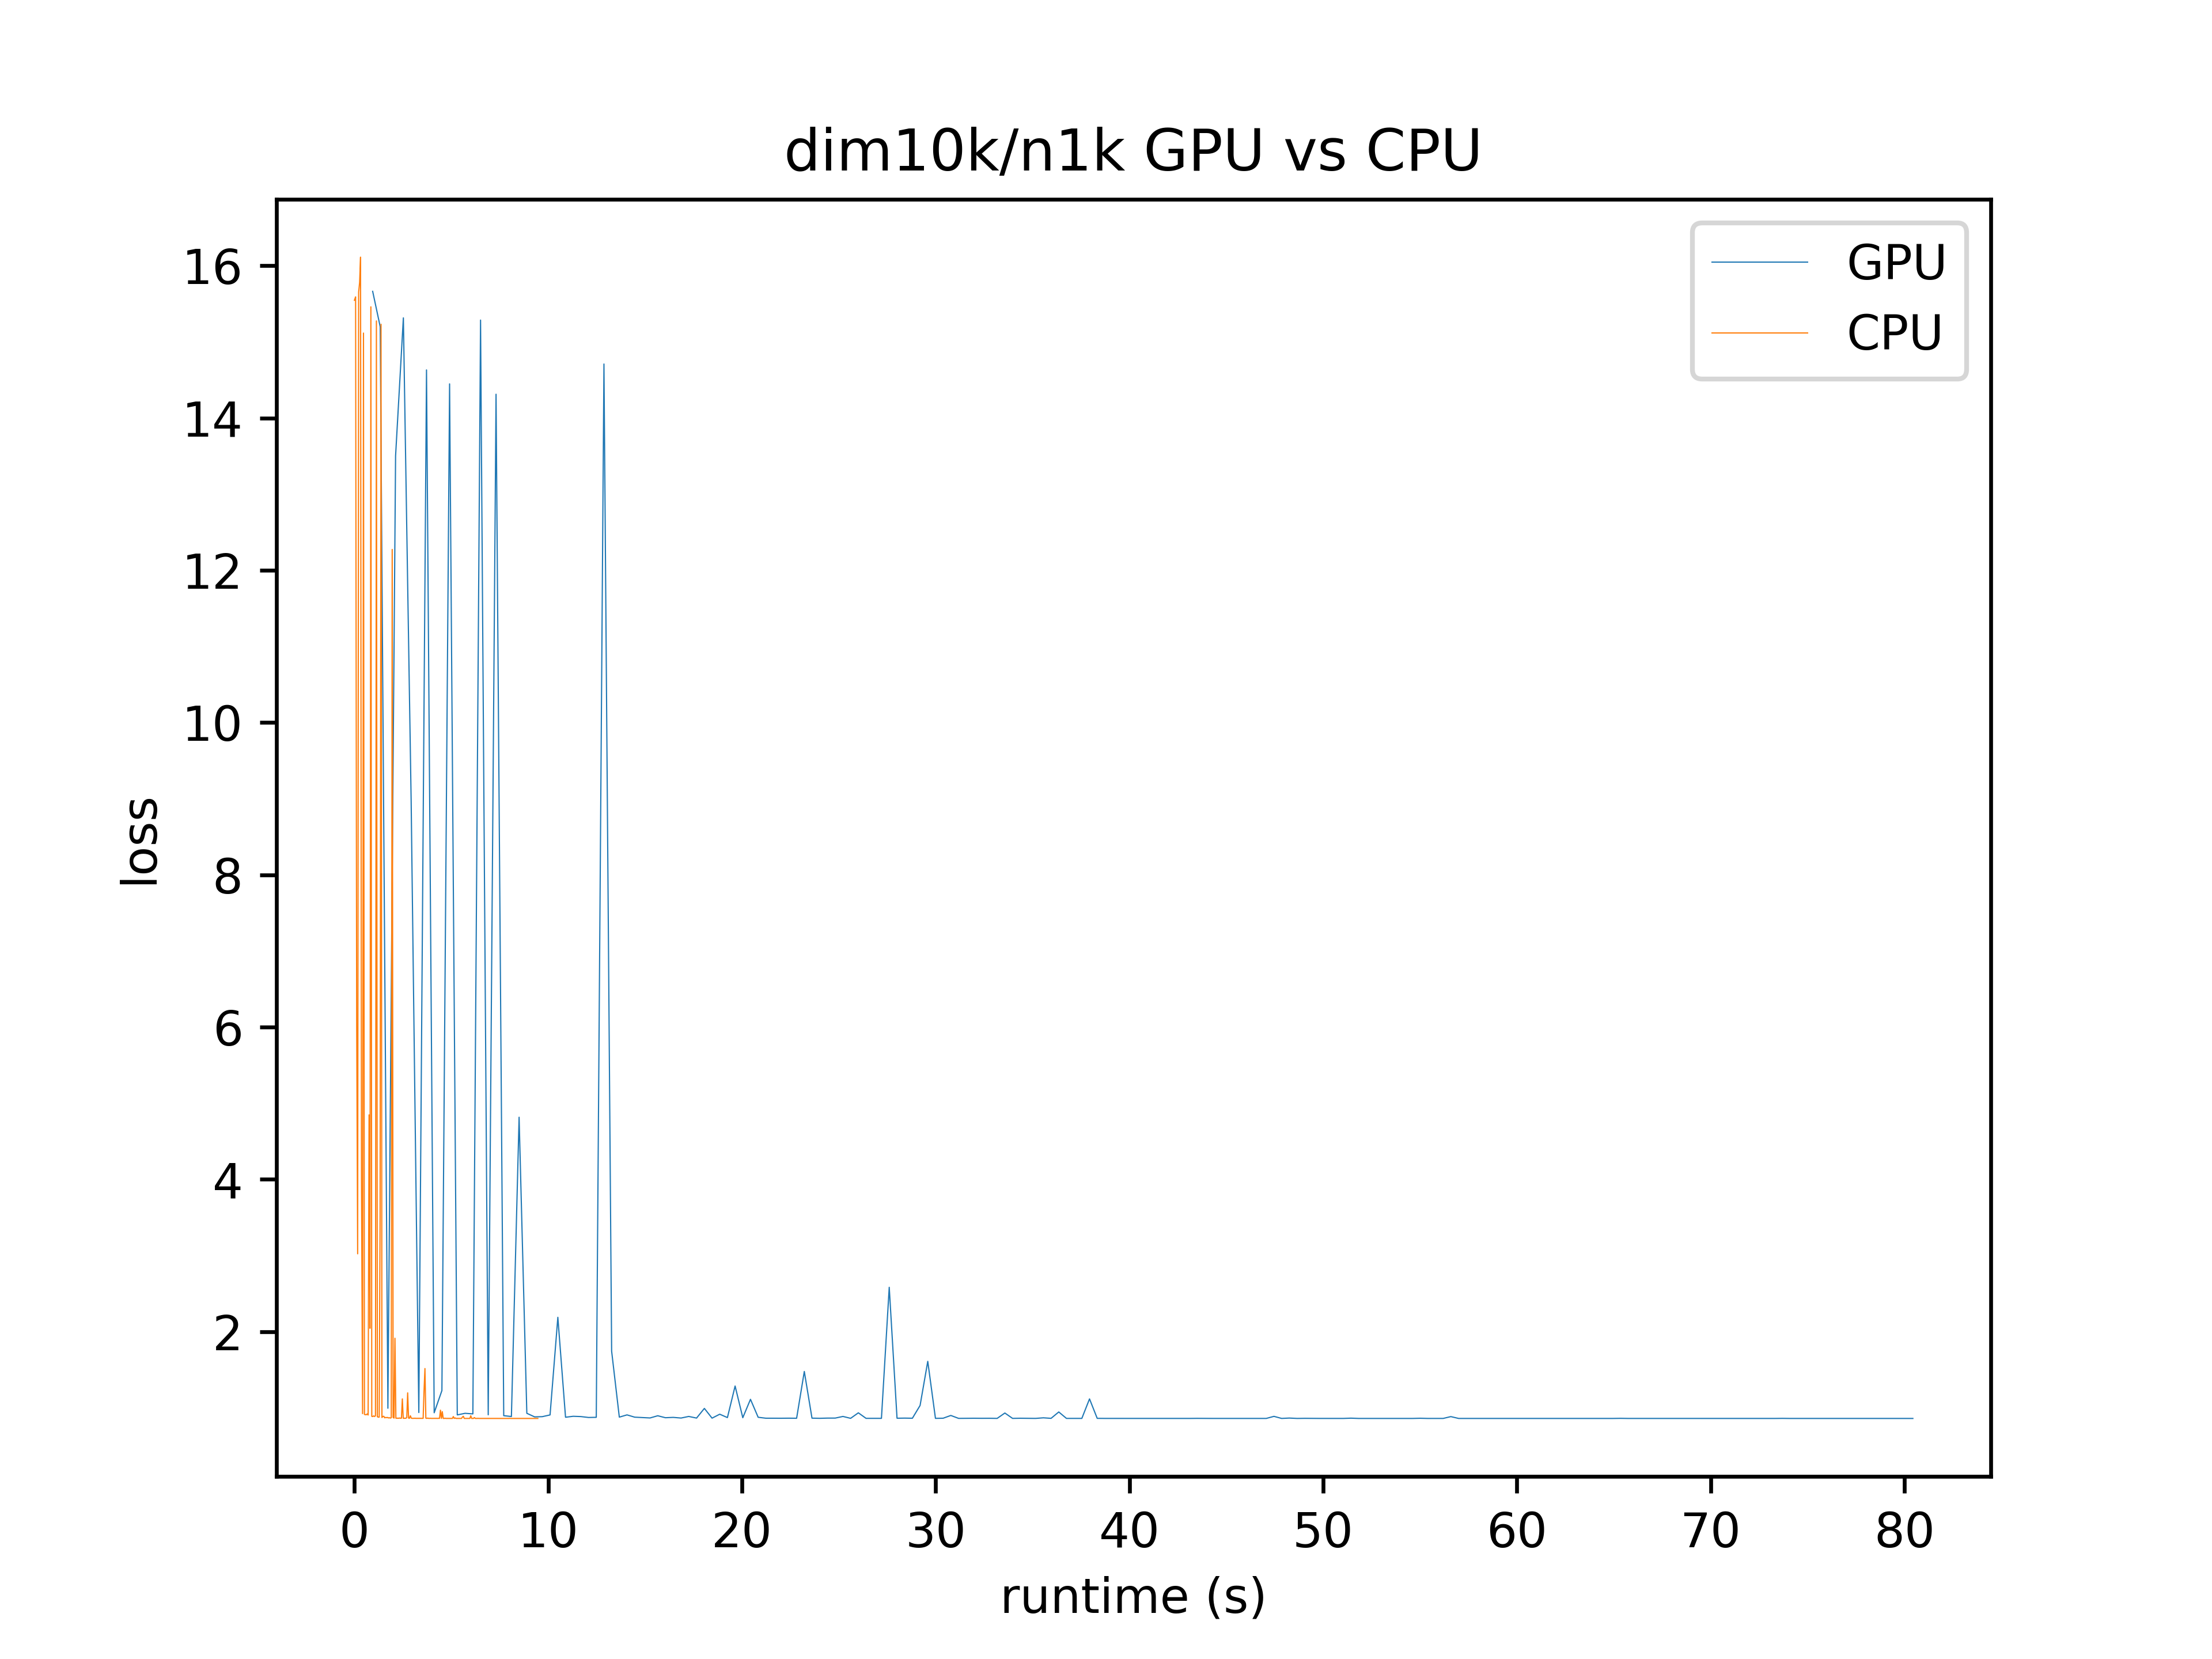
\includegraphics[scale=0.65]{dim10k_CPU_GPU}
  \caption{Comparison of training loss for generated data with 10,000
    features. The algorithms used are sequential CPU and sequential GPU.}
  \label{fig:10k}
\end{figure}

\begin{figure}
	  \label{fig:50k}
  \centering
  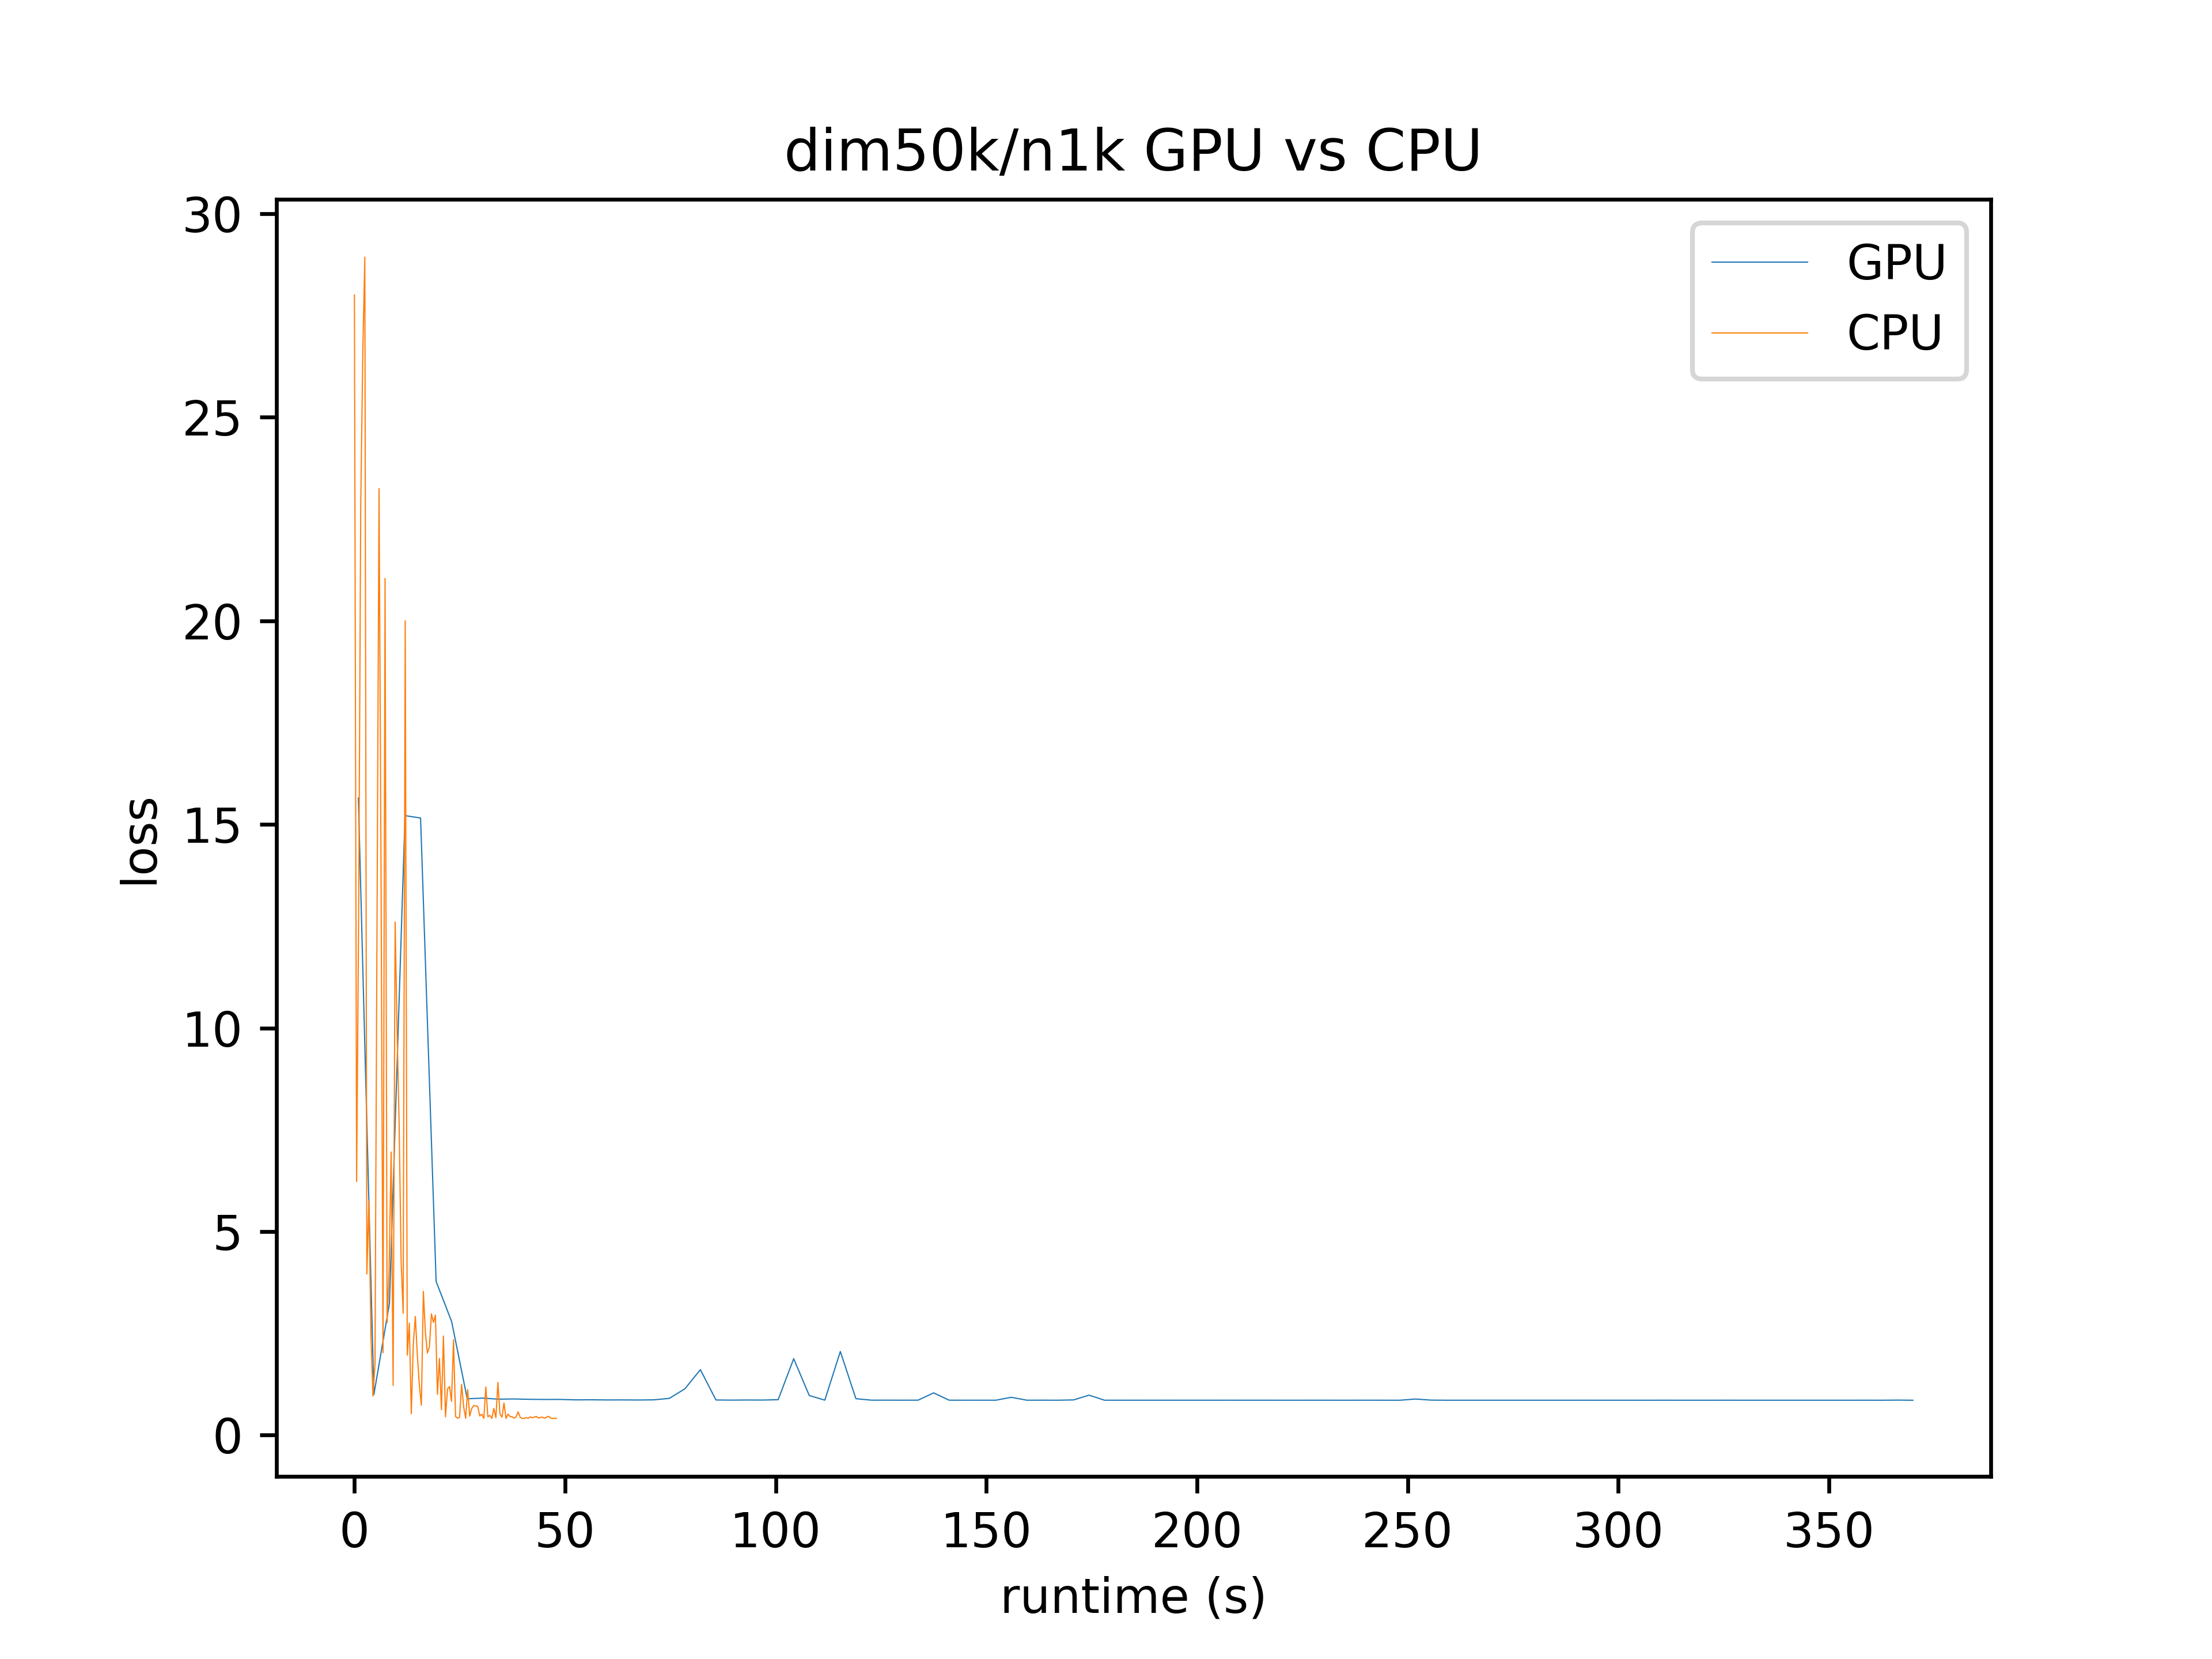
\includegraphics[scale=0.65]{dim50k_CPU_GPU}
  \caption{Comparison of training loss for generated data with 50,000
    features. the algorithms used are sequential CPU and sequential GPU.}
  \end{figure}

As expected, as the dimension of the feature space increases (Figure
\ref{fig:50k}), we see an improvement in the sequential GPU version relative to
the sequential CPU version. This is because the GPU implementation can more
efficiently handle vector dot product as the dimension of the vector
increases.
% Unfortunately, as we will discuss in the following sections, there
are other limiting factors preventing us from achieving ideal performance.
  
\section{Discussion of Experimental Results}
\subsection{Sequential GPU}
In the sequential SDCA (Algorithm \ref{sequentialSDCA}), for the hinge loss with $\ell_2$ regularization, the line 4 has a closed-form solution, so does the line 7 for distributed SDCA (Algorithm \ref{distributedSDCA}). Specifically, the line 4 for Algorithm \ref{sequentialSDCA} can be written as
\begin{equation*}
    \Delta\alpha_i=y_i\max\left(0,\min\left(1,\frac{1-x_i^\top w^{(t-1)}y_i}{\|x_i\|_2^2/\lambda n}+\alpha_i^{(t-1)}y_i\right)\right)-\alpha_i^{(t-1)}.
\end{equation*}
Suppose the dimension of $x_i$ is $n$, then the vector product $x_i^\top w^{(t-1)}$ spends $O(n)$ time. When $n$ gets larger, the GPU gets more dominating advantage over the CPU, so the experiment is consistent to our theory.
\subsection{Distributed GPU}
We didn't provide experimental results for distributed GPU version of SDCA, so now we provide some discussion about it. Theoretically speaking, $m$ (the number of samples in a mini-batch) controls the tradeoff between the computation on each machine (process), while in our case refer to GPU thread, and the communication cost over machines (processes)~\cite{yang2013trading,yang2013analysis}. When $m$ is small, the communication cost decreases when $m$ increases. However, we only have one GPU available so we can only take $m$ to be 1, which makes the communication cost prohibitively high. 

\section{Lessons Learned}
We learned a lot about what can go wrong and what considerations need to be
made when carrying out low-level implementations of machine learning
algorithms. It was surprising how big of a difference some of these
optimizations made (for example, memory allocations). If we were to start over
(which would probably be a good idea if this work were to continue), we would
make two major changes. First, we would create a data wrapper class to handle
all the synchronization work in a more intelligent fashion. Second, we would
take advantage of cuBLAS, a library of highly optimized CUDA kernels for
various linear algebra operations. Not only are the cuBLAS kernels better
optimized in terms of implementation, they also can better handle making thread
and block allocations on the GPU. It was a mistake not using this from the
beginning, but it was a lesson well-learned.

\section{Conclusion}
While our results were not what we were hoping for, we firmly believe there is
promise in this approach. The failure of our implementation is more due to lack
of low-level optimizations and smart memory usage than it is a failure of the
approach in general. This is seen by looking at the improvements in the GPU
algorithm runtimes for both sequential and distributed implementations as we
increased the size of the mini-batch. We believe further work on this topic is
merrited, both from theoretical and implementation point-of-views.

%\section{The Proposed Work}
%We will approach this problem from both theoretical and implementation
%perspectives. On the theoretical side we hope to make guarantees on convergence
%of our proposed approach, while on the implementation side we hope to build a
%scalable system that can take advantage of its hardware as well as work in a
%distributed setting.
%
%\subsection{Theory}
%We will try to establish the convergence result of the
%proposed asynchronous distributed SDCA and analyze the tradeoff between
%computation and asynchronous communication.
%
\section{Future Work}
We plan on continuing to complete the work to get more efficient implementation of GPU programming. In this report, we didn't successfully derive the theory of an asynchronous version of distributed SDCA, and we plan on doing it in the future work. 


%\subsubsection*{Acknowledgments}
%
%Use unnumbered third level headings for the acknowledgments. All
%acknowledgments go at the end of the paper. Do not include
%acknowledgments in the anonymized submission, only in the final paper.

%\section*{References}

%References follow the acknowledgments. Use unnumbered first-level
%heading for the references. Any choice of citation style is acceptable
%as long as you are consistent. It is permissible to reduce the font
%size to \verb+small+ (9 point) when listing the references.
%
%\medskip
%
%\small
%
%[1] Alexander, J.A.\ \& Mozer, M.C.\ (1995) Template-based algorithms
%for connectionist rule extraction. In G.\ Tesauro, D.S.\ Touretzky and
%T.K.\ Leen (eds.), {\it Advances in Neural Information Processing
%  Systems 7}, pp.\ 609--616. Cambridge, MA: MIT Press.
%
%[2] Bower, J.M.\ \& Beeman, D.\ (1995) {\it The Book of GENESIS:
%  Exploring Realistic Neural Models with the GEneral NEural SImulation
%  System.}  New York: TELOS/Springer--Verlag.
%
%[3] Hasselmo, M.E., Schnell, E.\ \& Barkai, E.\ (1995) Dynamics of
%learning and recall at excitatory recurrent synapses and cholinergic
%modulation in rat hippocampal region CA3. {\it Journal of
%  Neuroscience} {\bf 15}(7):5249-5262.
%123~\cite{Bolte:2006:LIN:1328019.1328299},\cite{banerjee2007generalized}\cite{zhangcs14}\cite{shalev2016sdca}\cite{yang2013trading}
%123~\cite{Shalev-Shwartz2016a} is a good approach
\bibliography{courseProject}
\bibliographystyle{abbrv}
\end{document}
